\section{Preliminary Study}

\begin{figure}[!t]

  \centering
  \hspace*{-1em}

  \begin{minipage}{4in}
    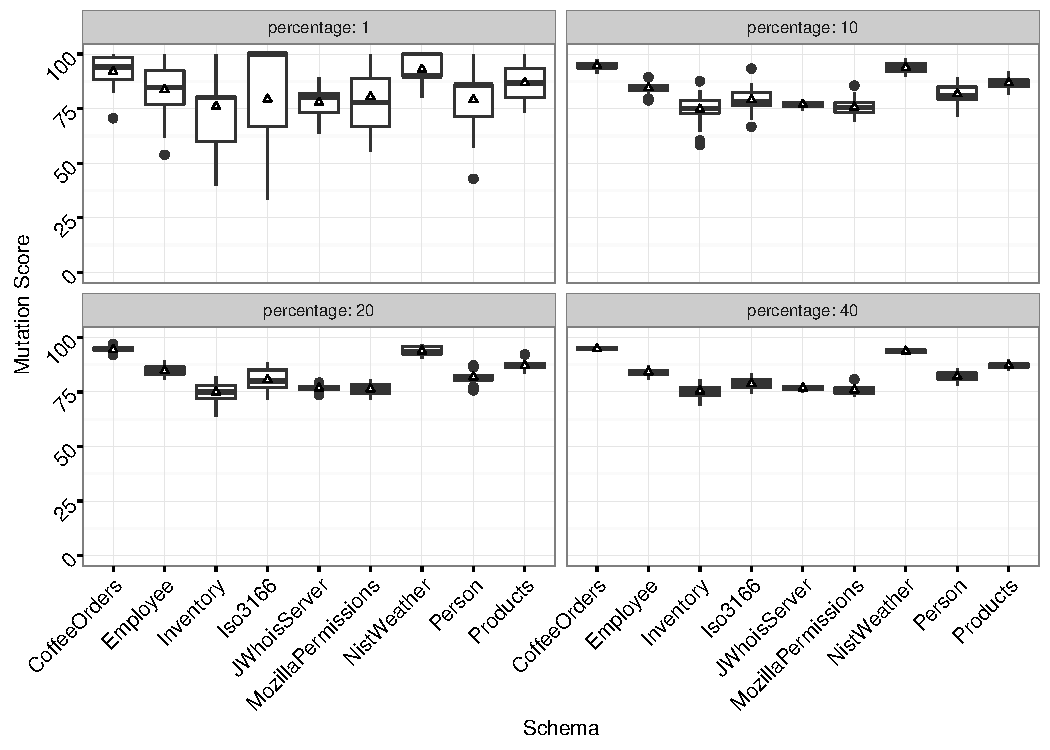
\includegraphics[scale = 0.5]{graphs/schema_vs_ms.pdf}
  \end{minipage}

  \caption{\label{fig:graph}Graph displaying mutation scores for database schemas.}

  \vspace{-1.8em}

\end{figure}


% GMK NOTE: All of this content is really about the design of the experiments and thus it has to be integrated into this
% section (currently, this is still rough content).

To display the effectiveness and the domain extensibility of \mr, we chose the nine schemas in Table~\ref{tbl:study-schemas}.
We chose these schemas because they range in triviality --- the total number of constraints ({\small$\sum$Constraints}).
This range in triviality allowed us to evaluate the effectiveness of reduction techniques performed by \mr~for schemas of varying
complexities.

Similar to Wong and Mathur in their studies~\cite{mathur1994empirical, wong1993mutation} where they conducted experiments using
mutant sampling with $x$ values ranging from $10\%$ to $40\%$, increasing by steps of $5\%$, we chose to analyse $x$ at $1\%$ and
then increase by $10\%$ intervals up to $90\%$. By lowering the granularity of the experiment to $10\%$ intervals instead of $1\%$
or $5\%$, we reduce the cost of performing retrospective analysis with \mr, while observing similar trends.


% CJM: to find the distance between original and reduced mutation scores
% this example below is just for an x value of 1

% d <- read_data("sqlite-avmdefaults.dat")
% d <- select_empirical_study_schemas(d)
% d <- select_normal_data(d)
% a <- analyse(d)
% pers <- c(1, 10, 20, 40)
% t <- dplyr::filter(a, method == "random_sampling", percentage %in% pers)
% t_filt <- dplyr::filter(t, percentage == 1)
% x <- dplyr::distinct(dplyr::select(a, original_mutation_score))
% c <- analyse_calculations(rs_filt_filt)
% y <- c$avg_reduced_mutation_score
% sub <- x - y
% max(sub) - min(sub)
%[1] 0.0336039

Figure~\ref{fig:graph}, a box-and-whisker plot showing the schemas analysed on the horizontal-axis and on the vertical-axis the
mutation scores of the reduced sets after random sampling at the following $x$ values: 1\%, 10\%, 20\%, 40\% (shown at the top
of a quadrant in a dark gray box). These $x$ values were chosen in this range because mutation scores start to become more accurate ---
closer to the mutation score of the original set. In the top-left quadrant of Figure~\ref{fig:graph}, $x$ is set to 1\%. At 1\% and
where RMSE ranges from $0.042$ to $0.139$, boxes are large, indicating that there is drastic variability in the mutation scores.
Additionally, in the same quadrant, lower extremes (represented by black dots) are more common and further from the lower quartile (the part
of the box below the horizontal line). Yet, the mutation scores observed of the reduced sets were
within $0.034$ of the original mutation scores.

Continuing to the next observed $x$ value of 10\%, RMSE ranges from $0.011$ to $0.053$, a
substantial increase in accuracy. At this same  $x$ value, Wong and Mathur observed that the mutation scores of reduced sets were
within $0.16$ from the mutation score of the original set~\cite{mathur1994empirical, wong1993mutation}. Using \mr~to retrospectively
perform random sampling with an $x$ value of 10\%, we observed mutation scores of reduced sets to be within $0.024$ from the original
set's mutation score.

As expected, reduced sets' mutation scores increase in accuracy with for $x$ of 20\% and 40\% with scores within $0.005$ and $0.006$,
respectively. It is acknowledged that these results, while substantially better than those found by Wong and Mathur
~\cite{mathur1994empirical, wong1993mutation}, may be specific to database schema mutation testing or even to this data.


